\section{Description du problème}\label{sec:DescProb}
Le mandataire, la \acrshort{Heig} ou plus particulièrement l'\acrshort{iAi}, souhaiterait disposer d'une maquette de démonstration pour les différents événements qui servent à présenter l'école. Elle aimerait pouvoir montrer un exemple classique de régulation avec un pendule inversé.
Il convient de développer, assembler et faire fonctionner la maquette du pendule inversé pour les événements à venir. Le pendule est libre en rotation autour d'un axe et l'équilibre doit être obtenu par déplacement linéaire selon un seul axe. Le pendule demandé est représenté dans la figure \ref{fig:Illustration}.

\begin{figure}[H]
  \centering
  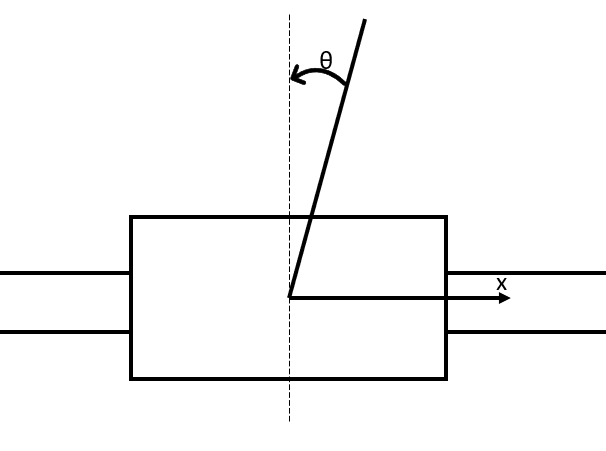
\includegraphics[width = 0.5\textwidth]{assets/figures/IllustrationPendule.svg.pdf}
  \caption{Illustration du pendule inversé demandé}
  \label{fig:Illustration}
\end{figure}

\section{Cas d'utilisation}\label{sec:CasUtil}
Lors des événements de la HEIG-VD, les visiteurs peuvent interagir avec la maquette de plusieurs manières. Une interface est présente et permet d'effectuer des opérations variées mais il est aussi possible de déstabiliser le pendule pour observer comment il arrive à se rattraper. Un affichage permettrait d'observer comment la régulation fonctionne en temps réel.
La figure \ref{fig:CasUtil} illustre ce cas d'utilisation typique.

\begin{figure}[H]
  \centering
  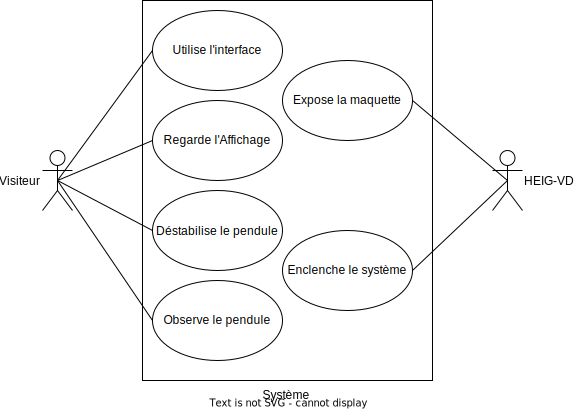
\includegraphics[width = 0.7\textwidth]{assets/figures/CasUtil.drawio.svg}
  \caption{Cas d'utilisation typique  du système à concevoir}
  \label{fig:CasUtil}
\end{figure}

\section{Analyse du besoin}\label{sec:AnalBesoins}
Suivant le cas d'utilisation illustré supra, les besoins identifiés de l'HEIG-VD sont exprimés au tableau \ref{tab:BesoinsHEIG}.

\begin{table}[H]
  \centering
  \caption{Besoins de l'HEIG-VD}
  \label{tab:BesoinsHEIG}
  \begin{tabular}{|l|l|}
    \hline
    \textbf{\#} & \textbf{Besoin}                                                   \\ \hline
    N1          & Intéresser de potentiels futurs   étudiants au métier d'ingénieur \\ \hline
    N2          & Disposer d'un système simple à   mettre en œuvre                  \\ \hline
    N3          & Assurer la sécurité des visiteurs   et des exposants              \\ \hline
    N4          & Présenter le domaine de la   régularisation numérique             \\ \hline
  \end{tabular}
\end{table}

Suivant le cas d'utilisation illustré supra, les besoins identifiés du visiteur sont exprimés au tableau \ref{tab:BesoinsVis}.

\begin{table}[H]
  \centering
  \caption{Besoins du visiteur}
  \label{tab:BesoinsVis}
  \begin{tabular}{|l|l|}
    \hline
    \textbf{\#} & \textbf{Besoin}                                    \\ \hline
    N5          & Se familiariser sur le sujet de la   régulation.   \\ \hline
    N6          & Se divertir à l'aide d'une   démonstration.        \\ \hline
    N7          & Découvrir le domaine des sciences   de l'ingénieur \\ \hline
  \end{tabular}
\end{table}

\section{Fonctions}\label{sec:Fonctions}
On détermine les fonctions suivantes dans le tableau \ref{tab:Fonctions} à partir des besoins de la HEIG-VD et des visiteurs qui sont indiqués dans le chapitre \ref{sec:AnalBesoins}, Analyse du besoin.

\begin{table}[H]
  \centering
  \caption{Fonctions du système à concevoir}
  \label{tab:Fonctions}
  \resizebox{\textwidth}{!}{%
    \begin{tabular}{|l|l|l|}
      \hline
      \textbf{\#} & \textbf{Fonctions système}                                                                     & \textbf{Besoin} \\ \hline
      F1          & Doit pouvoir tenir en équilibre                                                                & N5.1/N6.2       \\ \hline
      F2          & Doit pouvoir être autonome                                                                     & N5.1/N6.2       \\ \hline
      F3          & Doit pouvoir se mettre en équilibre tout seul depuis la position de repos                      & N5.1/N6.2       \\ \hline
      F4          & Doit permettre aux visiteurs d'effectuer des actions programmées sur le pendule.               & N5.1            \\ \hline
      F5          & Doit permettre aux visiteurs de déséquilibrer le système.                                      & N5.1            \\ \hline
      F6          & Doit expliquer aux visiteurs comment fonctionne le système.                                    & N5.1/N6.1       \\ \hline
      F7          & Doit pouvoir tenir sur une table.                                                              & N5.2            \\ \hline
      F8          & Doit pouvoir être alimenté facilement.                                                         & N5.2            \\ \hline
      F9          & Doit respecter les normes EN ISO 12100 de la SUVA \cite{NormeISO} sur la sécurité des machines & N5.3            \\ \hline
    \end{tabular}%
  }
\end{table}

Les fonctions sont disposées dans un diagramme FAST (c.f. Figure \ref{fig:AnalFAST}).

\begin{figure}[H]
  \centering
  \includegraphics[width = \textwidth]{assets/figures/AnalyseFAST.svg}
  \caption{Analyse FAST pour le pendule inversé}
  \label{fig:AnalFAST}
\end{figure}

\section{Exigences}\label{sec:Exigences}

\begin{table}[H]
  \centering
  \caption{Exigences de la solution retenue}
  \label{tab:Exigences}
  \resizebox{\textwidth}{!}{%
    \begin{tabular}{|l|l|l|l|}
      \hline
      \textbf{\#}                                                                                                             & \textbf{Exigence}                                                       & \textbf{Valeur attendue} & \textbf{Fonction} \\ \hline
      R1                                                                                                                      & Le système tient en équilibre tant qu'il est alimenté                   & Vrai                     & F7.1              \\ \hline
      R2                                                                                                                      & Le système retourne vers le centre lorsqu'il n'est pas perturbé         & Vrai                     & F7.2              \\ \hline
      R3                                                                                                                      &
      Le système est capable de se mettre en équilibre seul, à partir de sa position de repos                                 &
      Vrai                                                                                                                    &
      F7.3                                                                                                                                                                                                                                             \\ \hline
      R4                                                                                                                      & Temps d'amorçage de maximum 10 secondes                                 & \textless{}=10s          & F7.3              \\ \hline
      R5                                                                                                                      & Au moins 2 des 4 actions suivantes doivent être implémentées            & \textgreater{}=2         & F7.4              \\ \hline
      R6                                                                                                                      & Le pendule effectue un tour complet et reste équilibré                  & Vrai                     & F7.4              \\ \hline
      R7                                                                                                                      & Déplacement de bout en bout avec le pendule penché                      & Vrai                     & F7.4              \\ \hline
      R8                                                                                                                      & Le pendule s'arrête un moment et s'amorce d'un seul coup sec            & Vrai                     & F7.4              \\ \hline
      R9                                                                                                                      &
      Le chariot fait des mouvements de plus en plus amples pour rester en équilibre puis redevient graduellement plus stable &
      Vrai                                                                                                                    &
      F7.4                                                                                                                                                                                                                                             \\ \hline
      R10                                                                                                                     & Le système est capable de se rééquilibrer après une légère perturbation & Vrai                     & F7.5              \\ \hline
      R11                                                                                                                     &
      Les dimensions du système doivent rentrer dans un volume de 1400mm de largeur, 700mm de profondeur et 1000mm de hauteur &
      Vrai                                                                                                                    &
      F7.7                                                                                                                                                                                                                                             \\ \hline
      R12                                                                                                                     & Le système reste stable sur la table, même en fonctionnement            & Vrai                     & F7.7              \\ \hline
      R13                                                                                                                     & Le système peut être branché sur une prise 230V Suisse classique        & Vrai                     & F7.8              \\ \hline
      R14                                                                                                                     & Le système ne doit pas laisser la possibilité de se coincer les doigts  & Vrai                     & F7.9              \\ \hline
      R15                                                                                                                     & Le système possède un arrêt d'urgence                                   & Vrai                     & F7.9              \\ \hline
    \end{tabular}%
  }
\end{table}

\section{Etat de l'art}\label{sec:EtatArt}

\subsection{Segway}

L'exemple de pendule inversé le plus connu est le Segway \cite{Segway} qui utilise les perturbations des utilisateurs comme indications de la direction dans laquelle il est censé se diriger. Ainsi, en essayant de garder l'équilibre, il permet le déplacement de ses utilisateurs.

\begin{figure}[H]
  \centering
  \includegraphics[width = 0.3\textwidth]{assets/figures/Segway.png}
  \caption{Image d'un Segway \cite{Segway}}
  \label{fig:Segway}
\end{figure}

Ce genre de système n'est pas limité à un rail comme dans le projet courant. Ceci lui permet d'utiliser des roues pour effectuer le déplacement qui équilibre la personne.

\subsection{Pendule inversé}

Plusieurs projets de pendule inversé sont trouvables sur internet comme les deux suivants illustrés ci-dessous.
Le premier est un projet venant du site Instructables avec des éléments assez simples et peu chers visant à construire un pendule basique
pour introduire la régulation.

\begin{figure}[H]
  \centering
  \includegraphics[width = 0.8\textwidth]{assets/figures/PenduleInstructables.jpg}
  \caption{Image du montage du pendule inversé d'Instructables \cite{Instructables}}
  \label{fig:Instructables}
\end{figure}

On peut voir qu'une courroie est utilisée pour déplacer le chariot qui est guidé par des tubes en PVC et des roulements à billes. La mesure de l'angle, de la vitesse angulaire et de l'accélération angulaire du pendule se fait à l'aide d'un capteur d'inertie placé au bout de la tige.\\

Le pendule de l'entreprise Quanser est plus précis et possède une réponse plus rapide aux perturbations grâce au matériel plus coûteux utilisé pour le fabriquer. Il est aussi utilisé pour éduquer les utilisateurs sur la régulation bien qu'à un niveau plus avancé, spécifiquement dans un milieu universitaire.

\begin{figure}[H]
  \centering
  \includegraphics[width = 0.6\textwidth]{assets/figures/PenduleQuanser.png}
  \caption{Image du pendule inversé de Quanser \cite{Quanser}}
  \label{fig:Quanser}
\end{figure}

Celui-ci utilise deux encodeurs pour détecter la position angulaire de la tige et la position linéaire du pendule. Le système se déplace linéairement à l'aide d'un entrainement pignon/crémaillère et est guidé par une glissière.